\section{Aplicativo de dashboard}

\subsection{Descrição}
O aplicativo desenvolvido é uma dashboard que permite ao morador da casa ver os dados dos sensores em tempo real, enviar requisições para os módulos realizarem alguma ação, receber confirmações de que essas ações foram realizadas e gerenciar seus dispositivos - Morpheus e módulos. Essa dashboard foi implementada com base nas características dos PWAs apresentadas no capítulo de Arquitetura a fim de permitir uma boa experiência de usuário tanto em smartphones como em computadores.

\subsection{Requisitos}

\subsubsection{Requisitos funcionais}
\begin{description}

\item \textbf{Realizar cadastro, login e gerenciamento de informações pessoais}

\begin{itemize}
\item O usuário pode se cadastrar com seu email, nome e data de nascimento, criando também um nome de usuário e senha para acessar a dashboard.
\item O usuário pode realizar login usando seu nome de usuário e senha.
\item O usuário pode alterar as informações pessoais de seu cadastro.
\end{itemize}

\item \textbf{Gerenciar Morpheus}

\begin{itemize}
\item O usuário pode adicionar e remover controladores locais - Morpheus, sendo que para o cadastro basta adicionar o número de série do dispositivo.
\item O usuário pode configurar o Morpheus, especificando se deseja que mensagens que não puderam ser enviadas por problemas de conectividade devem ser mandadas assim que a conexão foi reestabelecida.
\end{itemize}

\item \textbf{Gerenciar módulos}

\begin{itemize}
\item O usuário pode adicionar e remover módulos, sendo que para o cadastro deve-se adicionar o número de série do dispositivo, relacioná-lo ao Morpheus que ouvirá suas mensagens, dar um nome ao módulo e seus relês e especificar o seu tipo.
\item O usuário pode configurar o módulo, especificando as configurações de conectividade, display e teste de auto-reset.
\end{itemize}

\item \textbf{Receber dados e enviar ações em tempo real}

\begin{itemize}
\item O usuário pode visualizar em tempo real os dados dos sensores de abertura, presença, temperatura, umidade e luminosidade do módulo básico.
\item O usuário pode visualizar o estado dos relês e enviar ações para ligá-los e desligá-los.
\item O usuário pode visualizar em tempo real os dados do estado do portão e do alarme do módulo de acesso.
\item O usuário pode, no módulo de acesso, enviar uma ação para abrir o portão usando uma senha.
\end{itemize}

\item \textbf{Alterar configurações avançadas dos módulos}

\begin{itemize}
\item O usuário pode receber confirmações de que ações sensíveis foram recebidas pelos módulos corretamente.
\item O usuário pode gerenciar o sensor de radiofrequência.
\item O usuário pode enviar uma ação para sincronizar a hora do módulo.
\item O usuário pode enviar uma ação para reiniciar o módulo (\textit{soft reset}).
\end{itemize}

\item \textbf{Visualizar estado das conexões}

\begin{itemize}
\item O usuário pode ver o status de sua conexão com o servidor da nuvem e da conexão de seus Morpheus com a nuvem.
\end{itemize}

\end{description}

\subsubsection{Requisitos não-funcionais}

\begin{itemize}
\item O aplicativo deve ser responsivo e totalmente funcional nos navegadores mais recentes em suas versões desktop e mobile.
\end{itemize}

\subsection{Tecnologias utilizadas}

Para criar a aplicação web que demonstra a funcionamento do Hedwig, foi escolhido o React\footnote{https://reactjs.org/}, biblioteca open source de JavaScript mantida pelo Facebook. O React é conhecido por facilitar o desenvolvimento de aplicações \textit{single-page}, renderizadas do lado do cliente, que permitem a atualização dinâmica da página de forma fluida e rápida, o que acaba enriquecendo a experiência do usuário. Possui uma linguagem declarativa e baseada em componentes, tornando-a altamente modularizável e reutilizável. Uma de suas características mais reconhecidas é o uso de um DOM virtual e um algoritmo que reconciliação que consegue identificar quais as partes da página precisam ser renderizadas a cada interação com o usuário \cite{reactdiff}, melhorando a performance e permitindo maior fluidez em animações e mudanças visuais.

Outro ponto interessante para a utilização do React é que, com a biblioteca React Native\footnote{https://facebook.github.io/react-native/} - uma extensão do React - é possível a geração de aplicativos nativos para iOS e Android. Assim, caso surja a necessidade de implementar uma nova funcionalidade que possui algum requisito que não pode ser contemplado por um \textit{Progressive Web App}, mas pode ser atendido por um aplicativo nativo, pode-se usar o React Native. Isso diminui a necessidade de retrabalho e dispensa a necessidade de estudo aprofundado das linguagens e ambientes de desenvolvimento tradicionais de projeto de aplicativos nativos.

A fim de facilitar a implementação das interações com o usuário, usamos juntamente ao React a biblioteca Redux\footnote{https://redux.js.org/}, um gerenciador de estado global. Dessa forma, pretendemos facilitar o compartilhamento de informações entres diferentes componentes. A motivação por trás do Redux é facilitar a leitura e atualização do estado da aplicação, que, em sites \textit{single-page} modernos, pode armazenar respostas do servidor, cache de dados e dados criados localmente que ainda não foram persistidos no servidor. O Redux é baseado em três princípios \cite{redux}:

\begin{itemize}
\item O estado é o ponto único de verdade.
\item O estado permite apenas a leitura - a única forma de alterá-lo é emitindo uma \textit{action}.
\item Alterações no estado devem ser feitas por funções puras - são os chamados \textit{reducers}, que recebem o estado anterior e uma \textit{action} e retornam o novo estado.
\end{itemize}

\begin{figure}
	\centering
	\caption{Diagrama de funcionamento do Redux}
  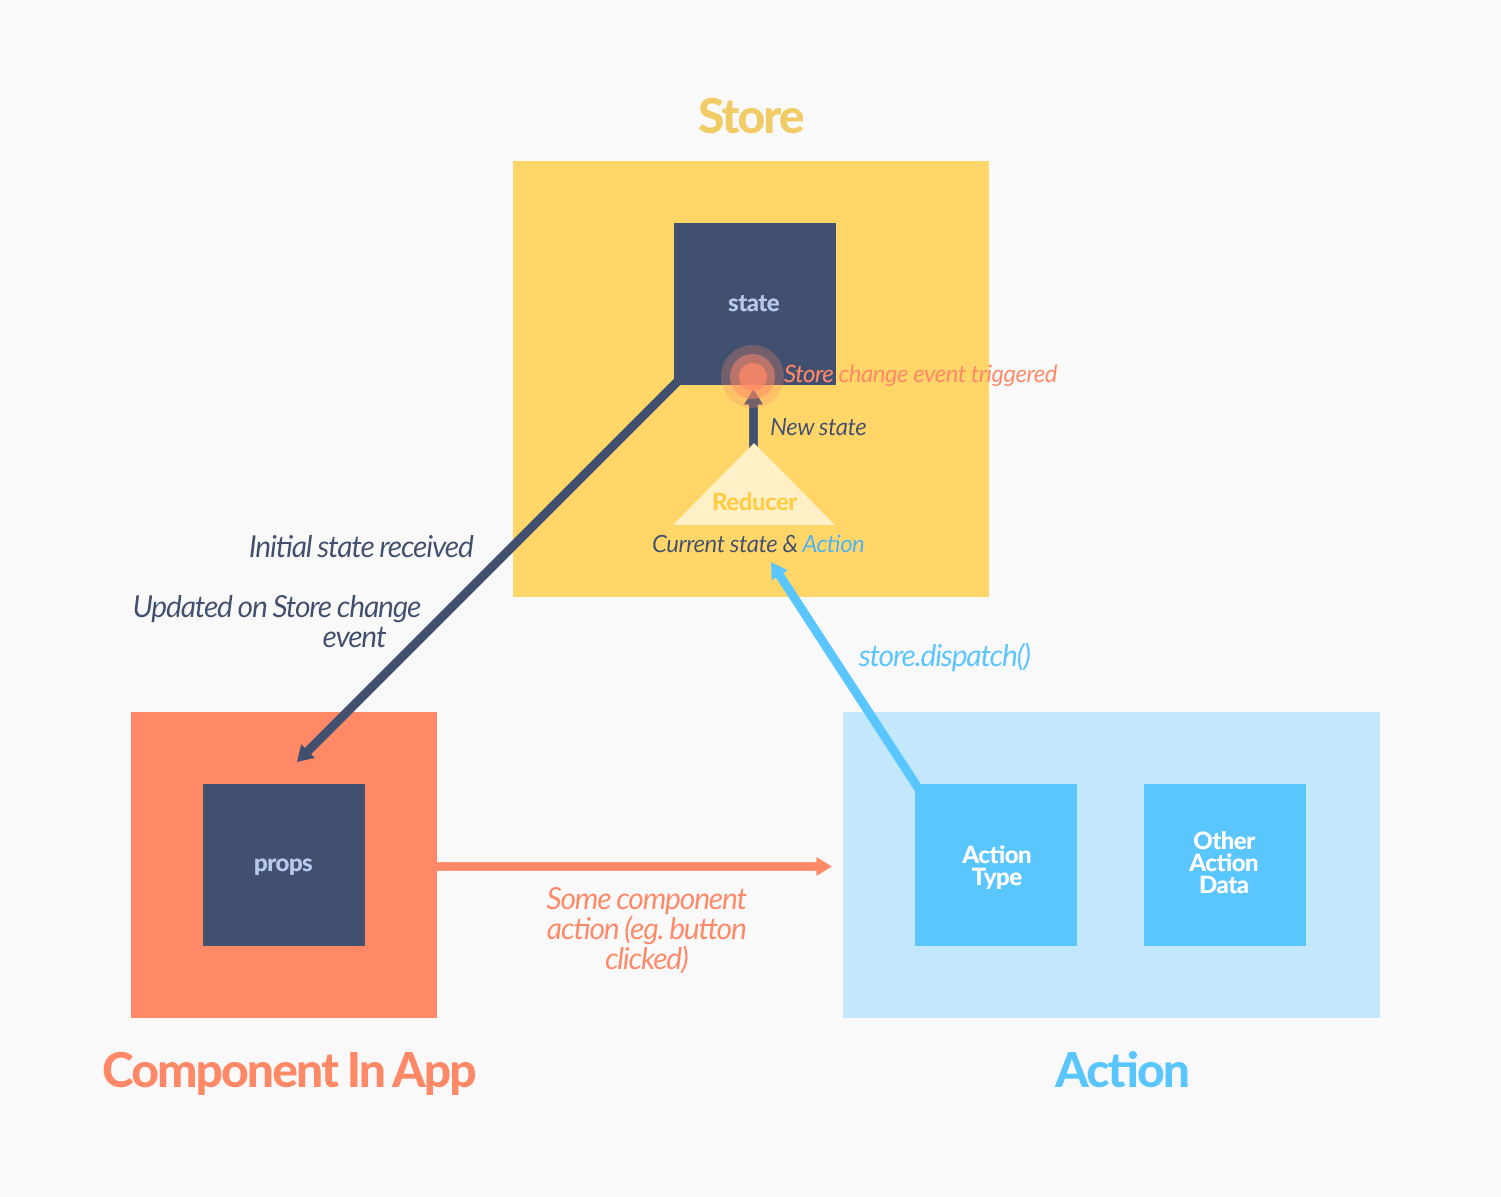
\includegraphics[width=\textwidth]{reduxFlowchart}
  \caption*{Fonte: \cite{reduxdataflow}}
\label{fig:reduxFlowchart}
\end{figure}

Para receber dados dos módulos em tempo real, foi usado um cliente do socket.io, framework que já foi discutido na seção do servidor na nuvem. O cliente de JavaScript já permite monitorar o status da conexão do aplicativo com o servidor, emitindo eventos em caso de desconexão ou reconexão. Assim, foi necessário criar \textit{listeners} para os eventos customizados que criamos para nossos protocolos.

Uma das vantagens em usar JavaScript para criar a view da aplicação é sua versatilidade, visto que é uma linguagem multi-paradigmas que suporta programação imperativa, declarativa e orientada a objetos \cite{mdnjs}. Outro ponto é que ela é usada tanto para desenvolvimento front-end como back-end, permitindo que o conhecimento acumulado na execução de um projeto ajude no outro.

Para aproveitar as funcionalidades e facilidades sintáticas das especificações mais recentes de JavaScript, usamos Babel\footnote{https://babeljs.io/}, um compilador capaz de converter as sintaxes novas e substituir as funções ainda não suportadas pelos navegadores com auxílio de \textit{polyfills}. Muitas vezes, é usado o termo transpilador para referir-se ao Babel, visto que é um compilador de JavaScript para JavaScript, não deixando de emitir como saída uma linguagem de alto-nível. Assim, é possível usar ES6 sem se preocupar com a compatibilidade do aplicativo com os navegadores que ainda não implementaram essa especificação completamente.

Para agilizar o desenvolvimento e prevenir falhas, usamos o \textit{linter} dedicado a JavaScript ESLint\footnote{https://eslint.org/}. \textit{Linter} é uma ferramenta para verificar o código e identificar erros de programação ou inconsistências de estilo \cite{linter}, o que possibilita produzir programas mais consistentes e menos suscetíveis a bugs.

Por fim, a pipeline de desenvolvimento do cliente usa o Webpack\footnote{https://webpack.js.org} como \textit{module bundler}. O Webpack cria gráficos de dependência de todos os componentes da aplicação web - imagens, folhas de estilo, scripts - e então os processa transformando-nos em \textit{bundles} ou pacotes, que nada mais são que arquivos estáticos.

\subsection{Interface}

\subsubsection{Identidade visual}

Para facilitar o desenvolvimento, foram usados os componentes do Material Design\footnote{https://material.io/} da Google, que satisfazem várias necessidades básicas e casos de uso da criação de interfaces modernas. Para distinguir cada tipo de módulo, foram usados ícones e paletas de cores distintas.

\subsection{Interações}

\subsubsection{Dados}

Dados provenientes dos sensores dos módulos são atualizados em tempo real por meio de eventos do socket.io. Para situar o usuário, o instante de tempo em que a mensagem do módulo foi enviada fica visível no fim na página. Caso seja detectado que a conexão com o Morpheus se perdeu, isso é mostrado explicitamente pela dashboard a fim de evitar que o usuário olhe dados antigos demais.

\subsubsection{Ações}

Ao enviar uma ação, o estado local do aplicativo não muda até que seja recebida uma nova mensagem de dados ou de confirmação. Isto é, se um relê está ligado e o usuário pede para desligá-lo, o aplicativo só vai mostrar que o relê desligou quando o módulo o avisa disso. Isso evita que o aplicativo entre em estados inconsistentes com os módulos.

\subsubsection{Conectividade}

O aplicativo possui um indicador no canto superior direito indicando o status da conexão. Ele pode assumir três estados:

\begin{itemize}
\item Aplicativos e todos os Morpheus do usuário estão devidamente conectados ao servidor na nuvem
\item Aplicativo está devidamente conectado ao servidor na nuvem, mas pelo menos um dos Morpheus não
\item Aplicativo não está conectado ao servidor na nuvem
\end{itemize}

Além disso, caso o aplicativo perca conexão com a nuvem, são emitidas notificações na parte inferior da tela. São realizadas 10 tentativas de reconexão e o resultado - positivo ou não - também aparece como um alerta na tela. Caso não haja sucesso em nenhuma das 10 tentativas, o usuário é aconselhado a atualizar a página.

\subsubsection{Aplicativo na tela inicial do dispositivo móvel}

Usando um arquivo de manifesto, foi possível configurar como o aplicativo aparece na tela inicial de um dispositivo móvel como um smartphone. Diminuindo o número de passos para o usuário acessar o aplicativo o encoraja a usá-lo mais vezes, além de criar uma sensação parecida com a de um aplicativo nativo.

\subsection{Publicação}

O aplicativo foi publicado com o serviço Surge\footnote{https://surge.sh/}, que permite a hospedagem de websites estáticos e oferece um domínio customizado. O Surge possui uma aplicação de linha de comando que permite a publicação de um diretório de arquivos HTML, CSS e JavaScript de maneira rápida e sem extensiva configuração. A dashboard está disponível em \url{https://hedwig.surge.sh}.

\subsection{Segurança}

O Surge usa a comunicação via HTTPS por padrão, oferecendo o suporte básico a SSL. Dessa forma, os dados transmitidos entre navegador e servidor podem ser criptografados, permitindo uma maior segurança em operações como cadastro, login e recebimento dos dados dos sensores.
